% !TEX root = ../Tesis.tex
\chapter{Construcción del Modelo} 
\label{cap:construccion} 

Los modelos que a continuación se presentan son compuestos por la DWT y cada una de las redes que estudiamos en el capítulo anterior: la NARNN, con la arquitectura propuesta por Asmaa Y. Fathi, et. al. \cite{DWT-NARNN} por un lado, y la estructura planteada por Adusumilli, R. \cite{ML_SP} para la la red con células LSTM (Long Short-Term Memory neural network) (LSTMnn) y la red con células GRU (GRUnn), así como las redes que no cuentan con el pre-procesamiento de datos de la DWT. 

Para la implementación, se usará \textit{Python 3.11} \footnote{El repositorio con el código del proyecto se puede ver en \url{https://github.com/MiguelAngelLiera/Stock_Exchange_NN_PP}.} \footnote{Las especificaciones del software utilizado se pueden ver en \ref{ApC}.} pues su sintaxis simple y legible facilita la programación y comprensión del código, lo que agiliza el desarrollo de los modelos de redes neuronales. Además cuenta con una cantidad importante de módulos y marcos de trabajo específicamente diseñados para el desarrollo de aprendizaje profundo. Algunos de los más populares incluyen TensorFlow, PyTorch, Keras, y scikit-learn (que revisaremos más adelante). Cada uno de ellos los iremos mencionado a medida que se requieran. Otra ventaja de su versatilidad es que permite combinar el uso de bibliotecas específicas con otras funcionalidades propias del lenguaje, como manipulación de datos y visualización de resultados en un mismo entorno.

\newpage

\section{Descomposición de datos por DWT}

A partir de este punto, se usarán los datos de \textbf{ACTINVRB} para cada uno de los pasos en la construcción de este y el siguiente capítulo. En este sentido, es un buen conjunto para la evaluación de los modelos desde que vemos la caída del valor de las acciones desde finales de 2019 (A partir de las doscientas semanas), hecho que se acentúa durante el primer año de la pandemia causada por la COVID-19. En palabras de Pablo Duarte, Director de Análisis y Estrategia de ACTINVER: "...la pandemia agregó mayor incertidumbre a las expectativas de crecimiento nacionales, mermando el ánimo de los inversionistas ya cautelosos por la crisis sanitaria." \cite{oportunidades_Actinver} Esta característica nos permite evaluar cómo reaccionan las arquitecturas ante eventos anómalos.

\begin{figure}[h]
    \centering
    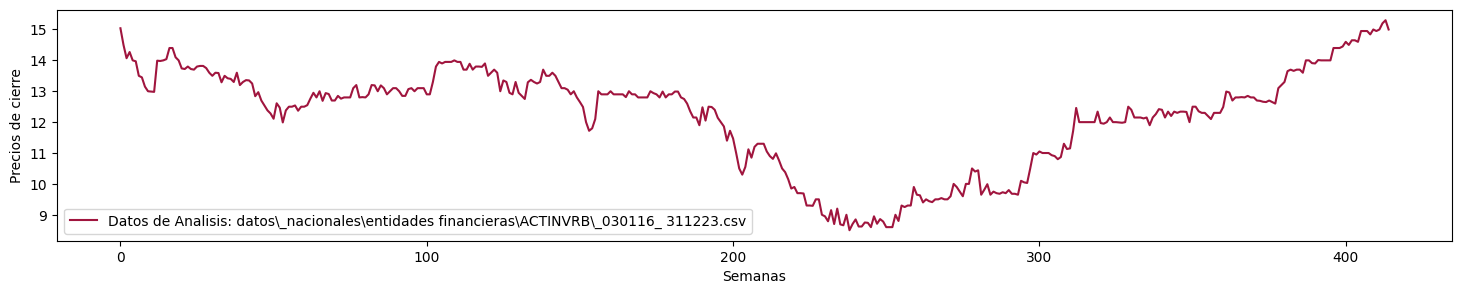
\includegraphics[width=1\textwidth]{Figuras/construccion_del_modelo/ACTINVR_030116_311223.png}
    \caption{Precios de cierre semanal de \textbf{ACTINVRB} del 1 de enero de 2016 al 31 de diciembre de 2023} 
    \label{fig:ACTINVRB}
\end{figure}

La biblioteca \textit{Pywavelets} \cite{pywavelets} cuenta con una implementación solida, eficiente y fácil de usar de algoritmos basados en ondículas tanto para análisis en tiempo continuo como en tiempo discreto. Proporciona una amplia gama de funciones para realizar transformaciones de ondícula y manipular coeficientes. Entre éstas podemos encontrar tanto para la descomposición de datos por DWT (función \texttt{dwt}) %\url{https://pywavelets.readthedocs.io/en/latest/ref/dwt-discrete-wavelet-transform.html#pywt.dwt}) 
 como para la reconstrucción de estos a partir de sus coeficientes (\texttt{idwt}, \texttt{upcoef}).

El primer paso de la descomposición es la elección de la ondícula madre. Se opta por una u otra dependiendo de las características de la serie de tiempo que se va a analizar. En general, debe ser en función del comportamiento de la serie original para que ésta pueda ser reconstruida o analizada. Para series que impliquen cambios no suaves y repentinos es recomendable usar \textit{bior3.5} \cite{DWT-NARNN}. Se trata de una ondícula madre que pertenece a la familia de ondículas biortogonales. La notación \textit{bior3.5} indica que tiene un filtro de paso bajo de longitud tres y un filtro de paso alto de longitud cinco en la descomposición, es decir, un filtro de tres coeficientes para la suavización (filtro de paso bajo) y un filtro de cinco coeficientes para la detección de detalles (filtro de paso alto). Así, nos da una buena representación de señales con cambios abruptos, lo que la hace útil en aplicaciones donde se requiere una alta capacidad de representación.

\begin{figure}[h]
    \centering
    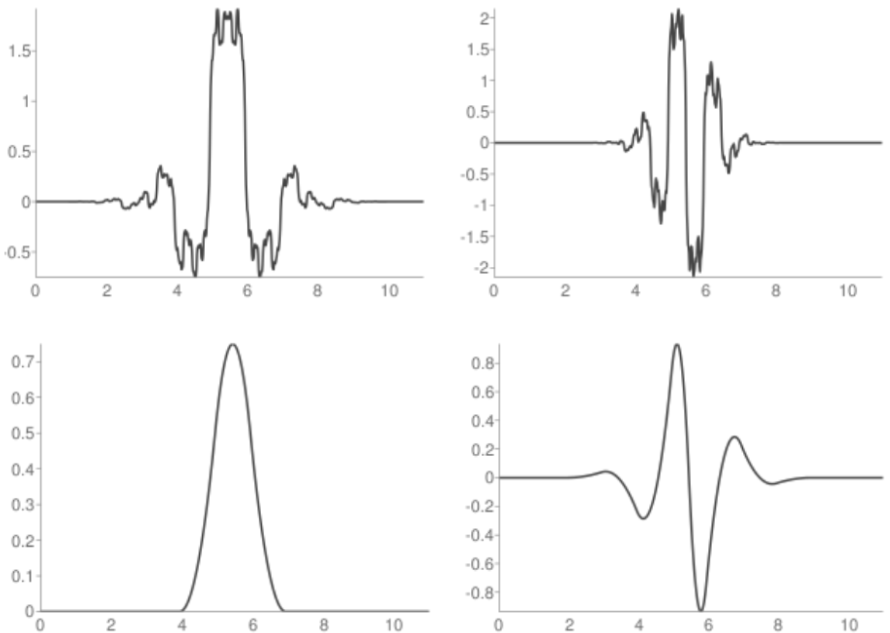
\includegraphics[width=0.7\textwidth]{Figuras/construccion_del_modelo/bior3.5.png}
    \caption{Funciones de descomposición (superior) y reconstrucción (inferior) de escala $\phi$ y de ondícula $\psi$. } 
    \label{fig:bior3_5}
\end{figure}

Para aplicar la DWT sobre los datos, es necesario realizar una extrapolación de los datos para que la descomposición en los extremos de la señal sea lo más precisa y limpia posible. Para nuestros fines, se escoge el modo \textit{symmetric} ya que refleja de mejor manera la descomposición en componentes de baja frecuencia.

\begin{figure}[h]
    \centering
    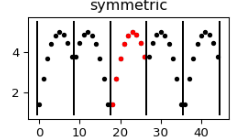
\includegraphics[width=0.5\textwidth]{Figuras/construccion_del_modelo/symmetric_pad_DWT.png}
    \caption{Extrapolación con modo \textit{Symmetric}.} 
    \label{fig:symmetric_pad}
\end{figure}

\newpage

\begin{figure}[h]
    \centering
    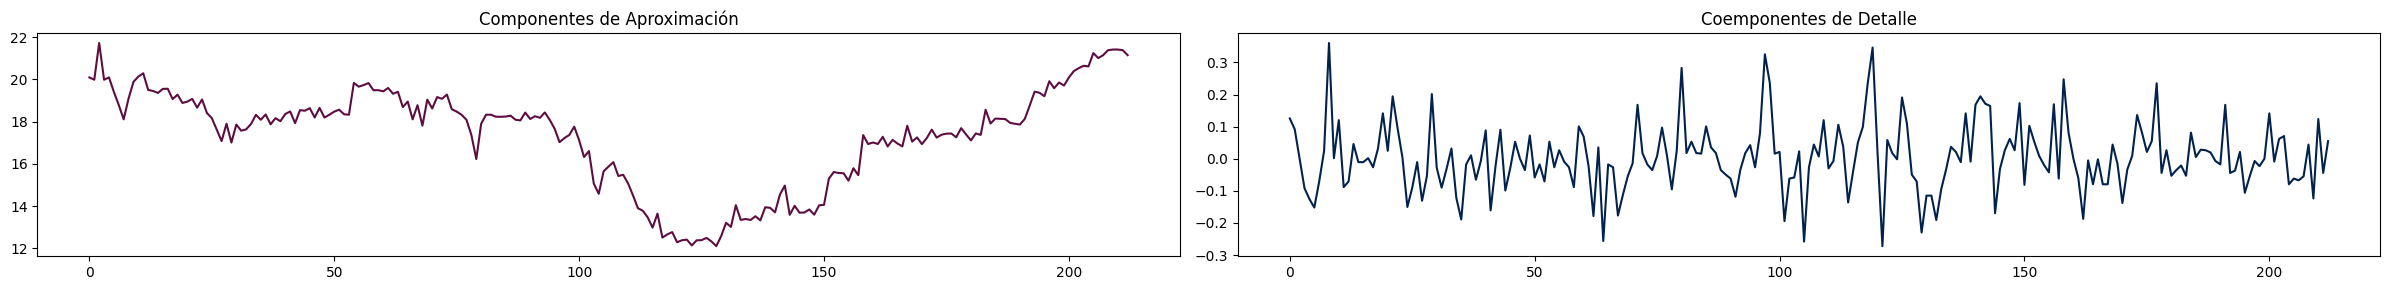
\includegraphics[width=1\textwidth]{Figuras/construccion_del_modelo/ACTINVR_DWT_lvl1.png}
    \caption{Componentes de Detalle y Aproximación de los datos de \textbf{ACTINVRB}.} 
    \label{fig:ACTINVRB_DWT_nivel1}
\end{figure}

Antes de continuar necesitamos dividir el conjunto de datos en entrenamiento (70$\%$) y prueba (30$\%$), para la fase del entrenamiento. Más adelante, durante el capítulo cinco \ref{cap:entrenamiento} se explica a detalle esta división.

\begin{figure}[h]
    \centering
    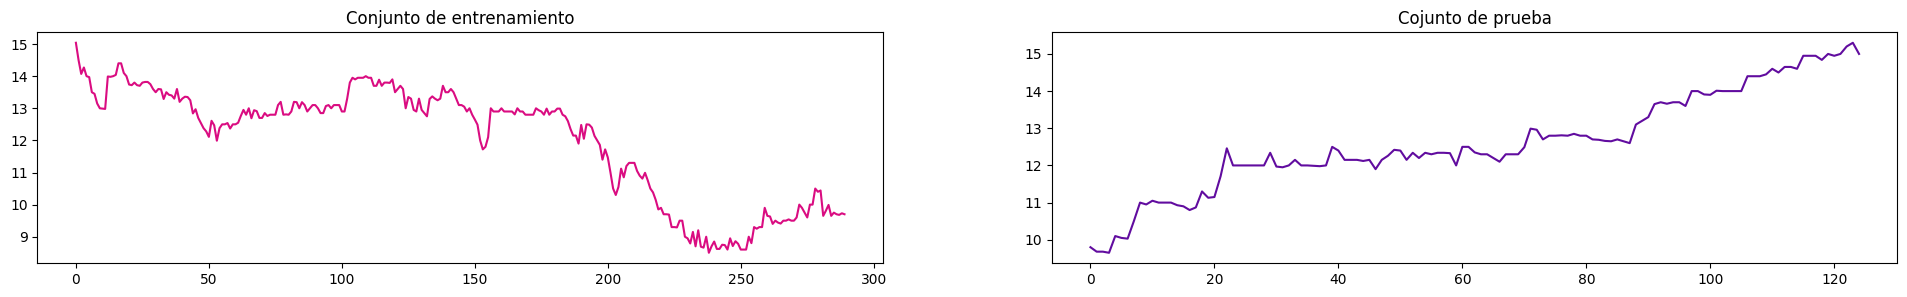
\includegraphics[width=1\textwidth]{Figuras/construccion_del_modelo/ACTINVR_entrenamiento_prueba.png}
    \caption{Conjunto de entrenamiento y prueba de los datos de \textbf{ACTINVRB}.} 
    \label{fig:ACTINVRB_entrenamiento_prueba}
\end{figure}

Para la eliminación del ruido de la señal, usaremos una descomposición en cinco niveles empleando el algoritmo piramidal que se mencionó en capítulos anteriores, atendiendo al hecho de suavizar la serie sin que pierda sus propiedades \footnote{La implementación de la descomposición multinivel de la señal por la DWT se puede encontrar en \ref{ApB}.}.

\begin{figure}[h]
    \centering
    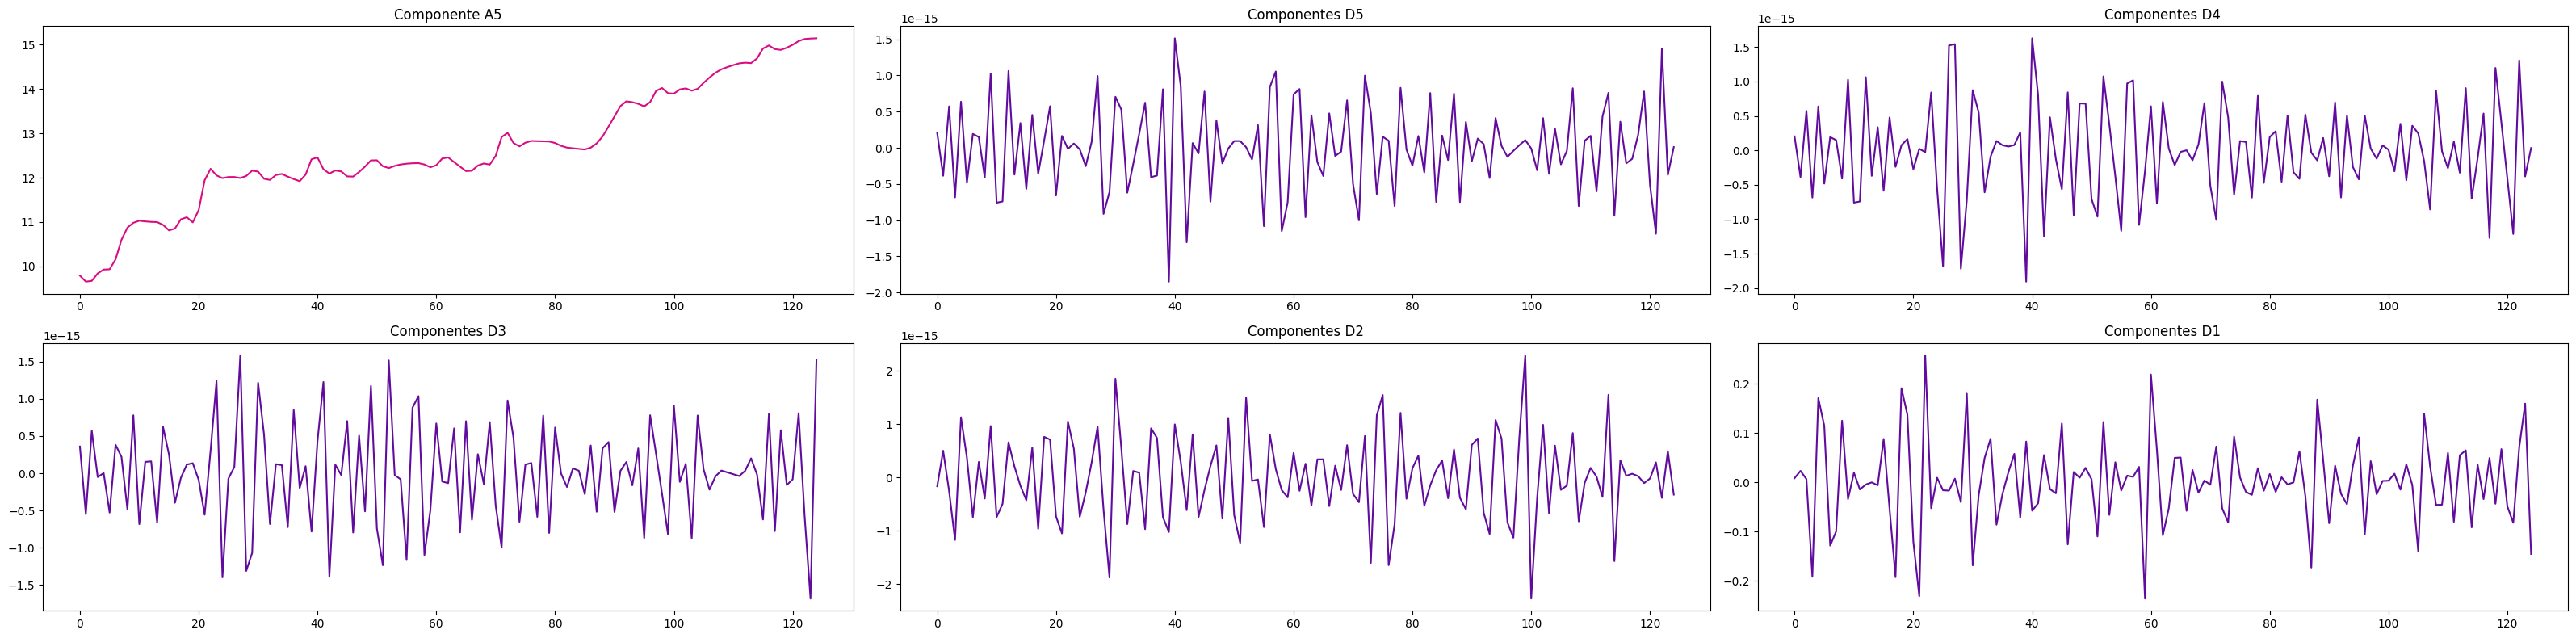
\includegraphics[width=1\textwidth]{Figuras/construccion_del_modelo/ACTINVR_prueba_DWT_lvl5.png}
    \caption{Componentes de detalle y aproximación en cinco niveles del conjunto de datos de prueba de \textbf{ACTINVRB}.} 
    \label{fig:ACTINVRB_prueba_DWT_nivel1_5}
\end{figure}

Para cada uno de estos componentes se creará una red NARNN, LSTMnn y GRUnn con el objetivo de pronosticar su comportamiento.

\newpage

\section{Modelo NARNN}

La arquitectura del modelo DWT-NARNN

\begin{figure}[H]
    \centering
    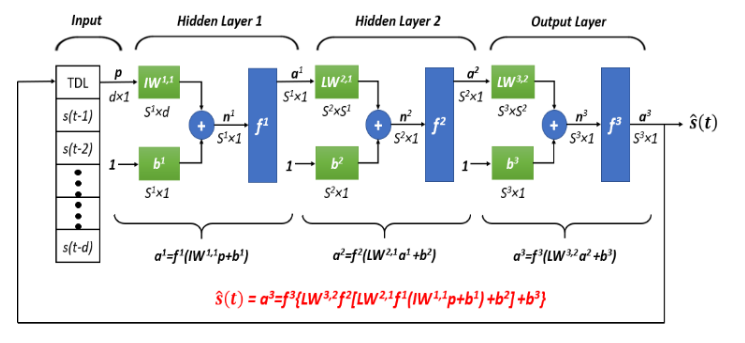
\includegraphics[width=0.8\textwidth]{Figuras/construccion_del_modelo/DWT-NARRN.png}
    \caption{Arquitectura NARNN (Recuperado de \cite{DWT-NARNN}).} 
    \label{fig:arquitectura_NARNN}
\end{figure}

En la figura \ref{fig:arquitectura_NARNN} podremos encontrar la arquitectura de la NARNN. Se trata de RNN con una Linea de Tiempo Retrasado (LTR) que representa los datos cierre de las ocho semanas anteriores a la predicción. También encontramos dos capas ocultas cada una con diez neuronas típicas y una última capa de salida con una sola neurona. Los sesgos de las neuronas en cada capa están representados por el vector $b$ y los respectivos pesos por los vectores $IW$ \textit{pesos de entrada} o \textit{input weights} y $LW$ \textit{pesos de capa} o \textit{layer weights} según la notación de Asmaa Y. Fathi, et. al. La función de activación en cada capa es la \textit{logaritmica-sigmoide}, \textit{tangente hiperbólica sigmoide}\footnote{Ambas funciones son versiones alternativas de la función sigmoide. Toman la composición de la primera en la segunda funcion, es decir:
\[
TanhSigmoide(x) = tanh\left[\dfrac{1}{e^{-x} + 1}\right]
\]\[
LogSigmoide(x) =log\left[\dfrac{1}{e^{-x} + 1}\right]
\]

Son efectivas para normalizar los datos y suavizar las pre-activaciones que reciben.
} y una función lineal respectivamente.

Para su implementación se utilizó la biblioteca \textit{pytorch} \footnote{Esta desición parte de la necesidad de crear un entrenamiento único (ya que se implementa el algoritmo LM para la parte entrenamiento) en comparación de las redes recurrentes.} \ref{ApB}.


\section{Modelo LSTMnn}

La red LSTMnn se toma la arquitectura:

\begin{figure}[H]
    \centering
    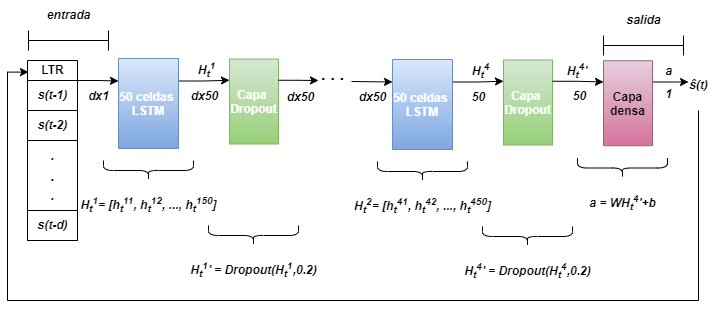
\includegraphics[width=0.8\textwidth]{Figuras/construccion_del_modelo/LSTMnn_arquitectura.png}
    \caption{Arquitectura LSTMnn.} 
    \label{fig:arquitectura_LSTMnn}
\end{figure}

La LSTMnn, al igual que la NARNN, presenta una LTR. Los ocho datos de entrada serán procesados por cuatro capas (células LSTM) con cincuenta unidades de salida cada una, y entre ellas cuatro capas de exclusión aleatorio o \textit{dropout} al veinte por ciento, de manera que esta cantidad de respuestas de la capa inmediata anterior se trunquen a cero para evitar el sobre-ajuste. Finalmente encontramos una capa densamente conectada con una sola neurona para la salida.

La implementación fue resuelta a partir de la biblioteca \textit{keras} \footnote{Gracias a que este marco de trabajo nos brinda una implementación solida de las LSTMnn y las GRUnn se decidió su uso.}. Se implementa la LSTMnn en \ref{ApB}.

\section{Modelo GRUnn}

Es una arquitectura par a la LSTMnn con la diferencia de que las capas con células LSTM son remplazadas por capas GRU, esto para mostrar una comparación equivalente y transparente entre el par de redes recurrentes. La red GRUnn se toma la arquitectura:

\begin{figure}[H]
    \centering
    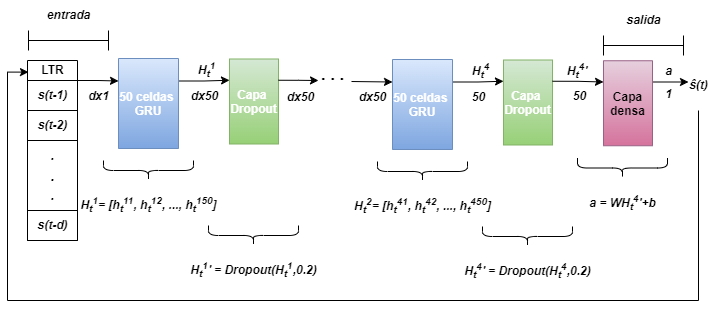
\includegraphics[width=0.8\textwidth]{Figuras/construccion_del_modelo/GRUnn_arquitectura.png}
    \caption{Arquitectura GRUnn.} 
    \label{fig:arquitectura_GRUnn} 
\end{figure}

La implementación fue resuelta a partir de la biblioteca \textit{keras}. Se implementa la GRUnn en \ref{ApB}.




